\section*{Mini-Project 2: A Two-Bit Adder}
\label{lab_two_bit_adder}

\fancypagestyle{interlude}[fancy]{%
	\fancyhead[LO,RE]{}
	\fancyhead[LE,RO]{\slshape \MakeUppercase{Mini-Project 2: A Two-Bit Adder}}
}
\addcontentsline{toc}{section}{\hspace{0.35in} \textbullet~Mini-Project 2: A Two-Bit Adder}
\pagestyle{interlude}

%\makelabheader %(Space for student name, etc., defined in master.tex)

\bigskip

\textbf{Background}

Logic gates are the fundamental building blocks of computer chips, and if you cram enough of them into a tiny chip, they can become tremendously powerful!  Your task in this Mini-project is to build an extremely modest example of this power: a circuit that performs addition on a pair of two-bit numbers.

Numbers in a computer are typically represented in base two by a series of ones and zeroes.  While base-ten numbers are represented by digits for each power of ten (e.g. ones, tens, and hundreds places, etc.), the digits in base-two numbers are for powers of two: ones, twos, fours, eights, sixteens, and so on.  The figure below shows how the number 125 can be written either in base ten as $100 + 20 + 5$, or in base two as $64 + 32+16+8+4+1$.

\begin{center}
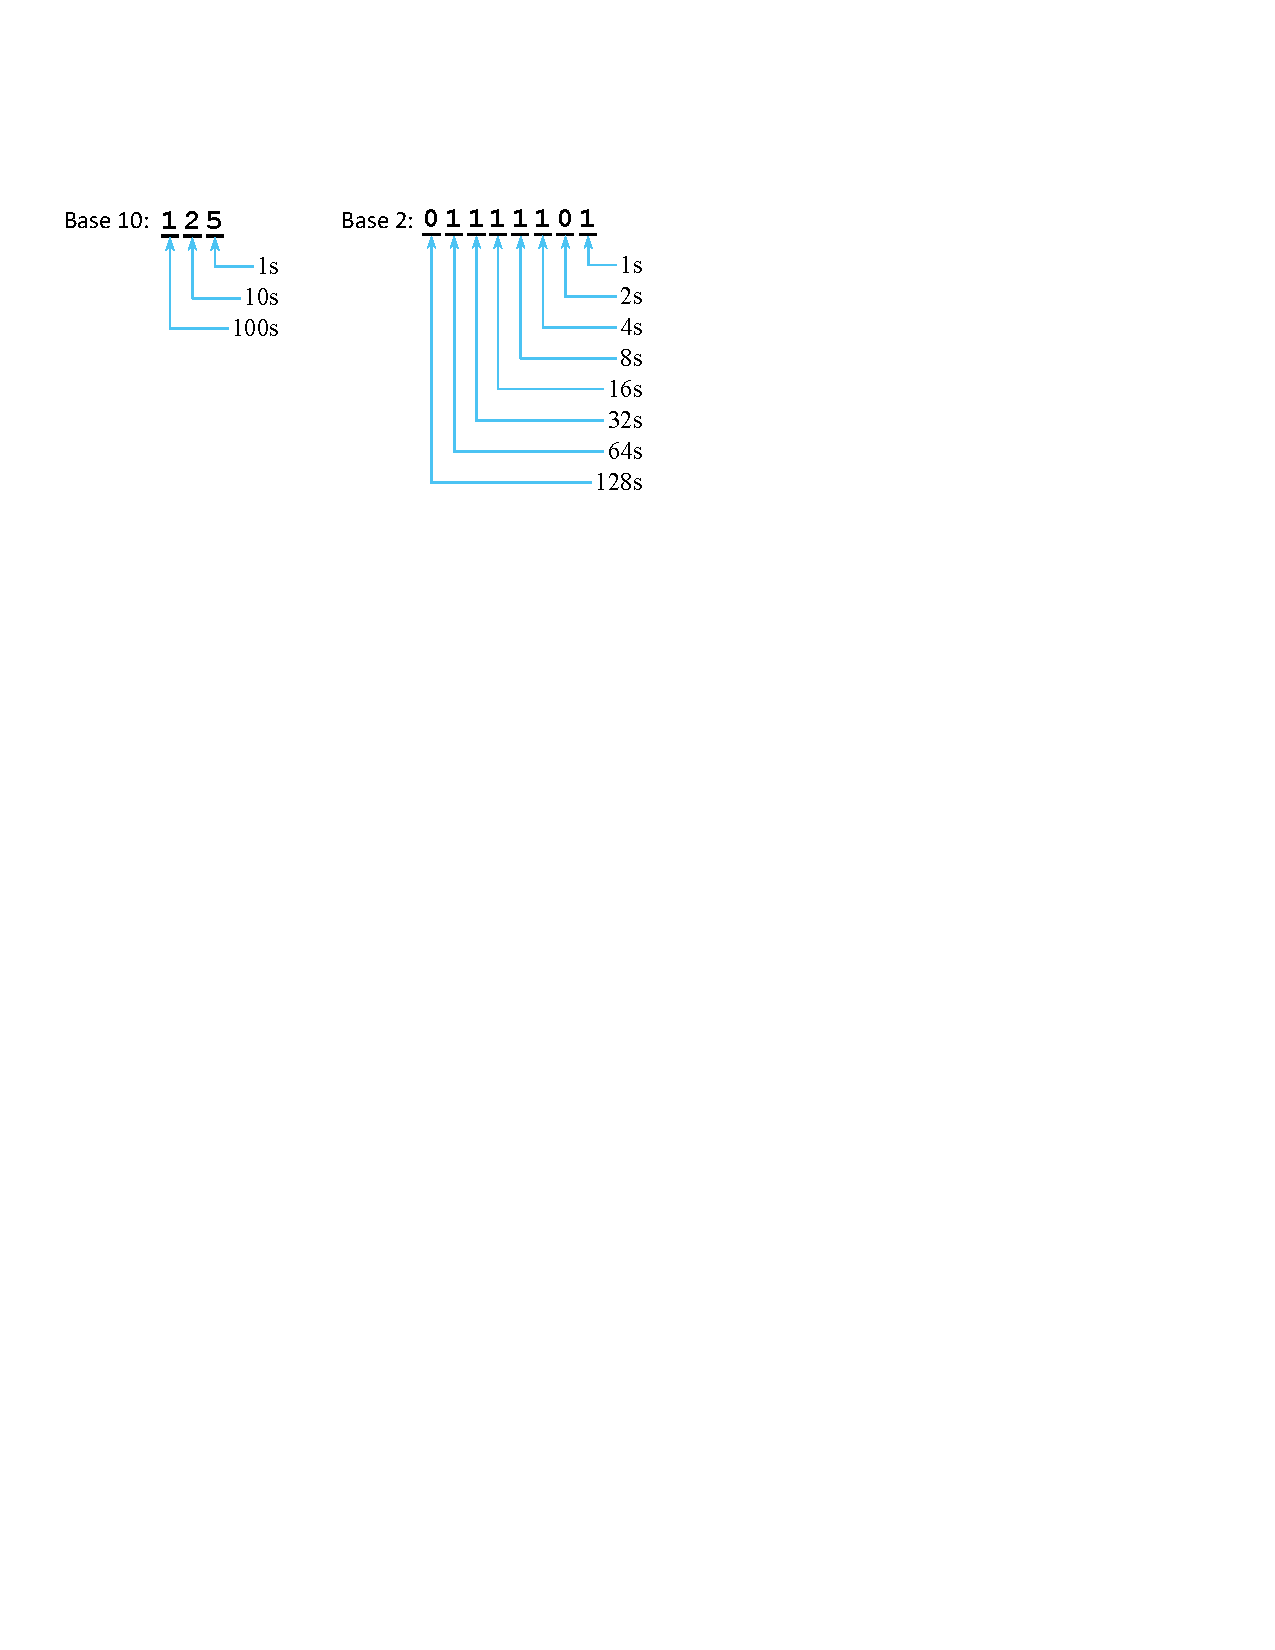
\includegraphics{digital_electronics/base_two.pdf}
\index{color_picture}
\end{center}

\textbf{Details and Hints}

The two numbers you will add in this project will each be limited to just two bits: a ones place and a twos place.  That is, each number will be either 0, 1, 2, or 3, represented by two input bits as 00, 01, 10, or 11.  Thus, your circuit will have a total of four logical inputs, each either 0 volts or 5 volts, representing a logical 0 or logical 1.  

The result of the addition will be a number from 0 to 6 that can be represented with three bits: the 1's, 2's, and 4's place.  Thus, your circuit will have three outputs ($S_1$, $S_2$, and $S_3$ in the figure below), each either 0 or 5 volts.  

How do you add two numbers in base two?  Exactly the same as in base ten: go digit by digit starting from the ones place, and ``carry the one'' when needed.

\begin{center}

\includegraphics{digital_electronics/addition_example.pdf}
\end{center}

In the base-two case above (again, your two numbers will only have two digits, not eight) the output $S_1$ is the sum of the inputs $A_1$ and $B_1$---either a 0 or a 1, and your job is to figure out the truth table.  However, if $A_1$ and $B_1$ are both 1, then $S_1 =0$, and you would also need to ``carry the one'' to the twos place.  Thus, the sum $A_1 + B_1$ actually has \textit{two} outputs: $S_1$ and $C_2$.  Moving on to the twos place, your next operation has three inputs: $C_2$, $A_2$, and $B_2$.

You can use any of the logic chips you have in your kits to make your two-bit adder.  Test your circuit using the logic switches on your board to control the inputs, and the logic indicators to view the outputs, and remember to show your instructor when you have it working.

